\section{Solution}
\subsection{Executing on GPU cluster and Timing}
We performed all our experiments on a remote GPU cluster as described in \ref{sec:system}.

The nodes in this cluster have no GL installed, therefore we could not run the given CPU application directly on any of those.
This required us to strip all GUI elements from the CPU implementation.

Due to the way the program was organized we were able to do this in a reasonable amount of time by just not compiling the GUI frame classes and removing the references to the GUI from the rest of the code.
Luckily, only the main method had references to the GUI, the rest of the program was free of GUI implementation details.

In GUI mode, the tool would run the entire algorithm each time a parameter changed.
Our new program runs the algorithm once, outputs the number of possible collisions left (split up into vector-face and edge-edge) after the execution of the \texttt{breakDown} function (we use these metrics to later compare the GPU implementation to the CPU implementation) and exists.

Another issue was how we would measure the time it took for our program to complete on both the CPU and GPU implementations.
Because the implementations work fundamentally different, this proved to be quite a challenge.

Our first approach was to count the number of processor clock ticks that have elapsed during the call to the \texttt{breakDown} function.
However, due to the asynchronous nature of CUDA kernel calls and the way clock ticks are calculated on POSIX compliant operating systems, we decided to use real elapsed time (using the \texttt{gettimeofday} function from \texttt{<sys/time.h>}).

When we switched to counting milliseconds we discovered that the real running time of the CPU implementation in our testing environment (as described in Section~\ref{sec:system}) was frequently below 1 millisecond, even on the highest data set that was available to us.
Due to this, we started looking in to ways to re-run the experiment multiple times to get a more meaningful number.
Unfortunately, this proved very difficult since there is a set-up algorithm that needs to be run before the \texttt{breakDown} function can get meaningful results.
The real running time of the \texttt{breakDown} function is about 0.5\% of that set-up function.
Because of this, the only way to get results is to run the set-up function an $n$ amount of times, then run the set-up plus the \texttt{breakDown} function $n$ times and subtract the running times to get an approximate time for the real running time of \texttt{breakDown}.

Running the algorithm multiple times was an even harder challenge for the GPU implementation.
Besides the previously mentioned set-up, the GPU implementation requires some extra set-up for CUDA.
This mostly consists of copying required data into the GPU device memory.
Unfortunately, where the actual running time of the algorithm on the GPU is again smaller than 1 millisecond, this copying can take over 1,200 milliseconds, even for small data sets.

When looking for more precise measures, we found out that the compiler on our machine also supported microseconds.
We were not able to find out a guarantee on how precise this was, but it seemed our best option.

In the end, we added a flag to the program that, if set, outputs the number of microseconds it took for the \texttt{breakDown} function to run and suppresses all other output.
For the CPU implementation, this time difference is calculated between the start and end of the \texttt{breakDown} function.
For the GPU implementation, it is calculated between the start of the CUDA threads and when they have \textbf{all} completed.
Note that we do not measure the time it takes to copy the required data in and out of the GPU device memory, as in a 'real' implementation, where the entire algorithm would run on the GPU, this data would already be available.

After that, we ran both the CPU and the GPU implementations of the program with the flag set $200$ times to generate enough samples (since we are not sure how precise the measurement in microseconds is).
With these samples, we construct two boxplots in the R program so we can easily spot if there are any significant differences in the running times of the CPU and GPU implementations.

An example of one of these graphs, in this case for the \texttt{bunny.txt} data set, is shown in Figure~\ref{fig:bunny_box}.

\begin{figure}
	\center
	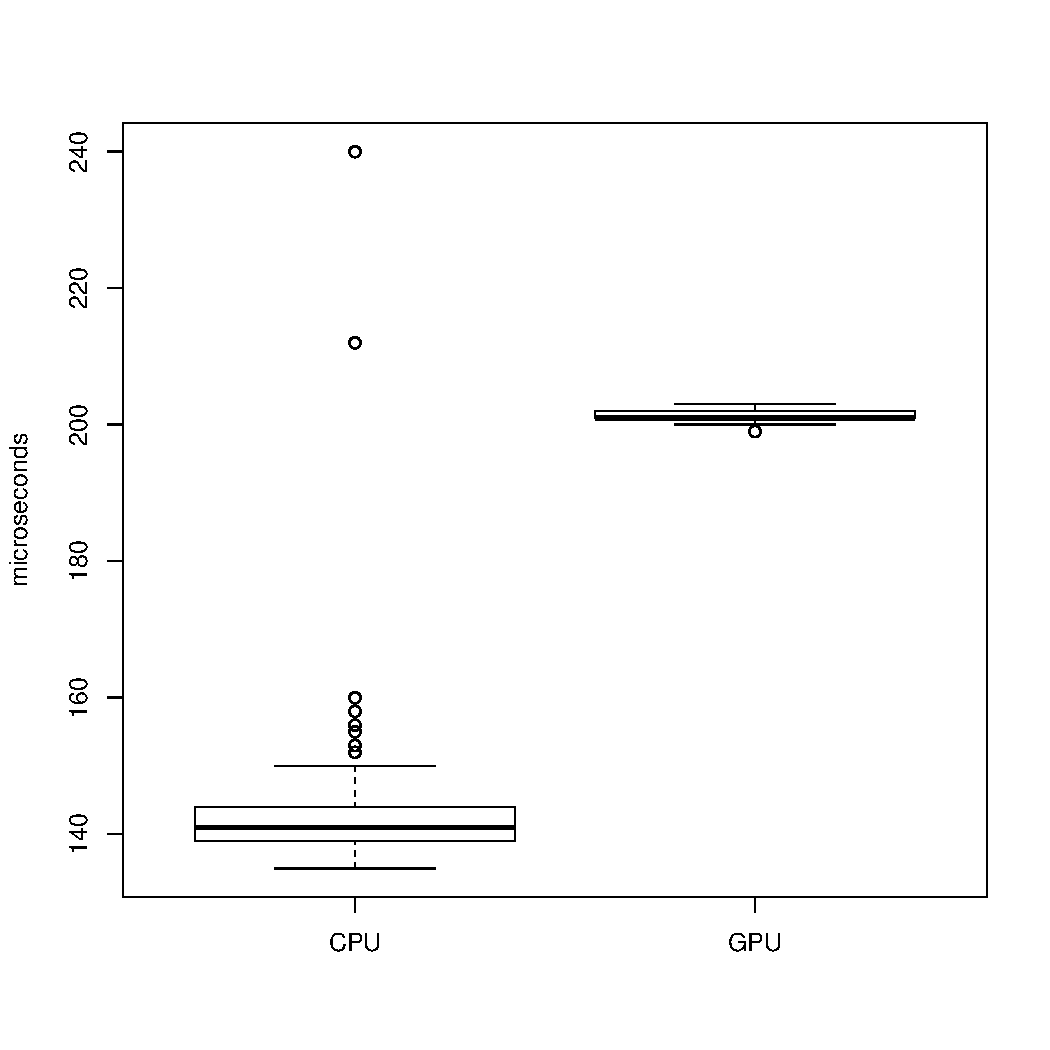
\includegraphics[width=0.5\textwidth]{results/bunny.pdf}
	\caption{Example boxplots for the \texttt{bunny.txt} data set}
	\label{fig:bunny_box}
\end{figure}

\subsection{Distribution over threads in CUDA}
The first approach to distribute the calculation over the threads in the GPU, is to let each thread do the calculations for one single face-face pair, to the corresponding vertex-face and edge-edge pairs. Figure \ref{fig:threaddist} gives an overview of this setup. We assign 256 threads per block, in a 16x16 matrix, and then have the number of blocks calculated as follows: for the x-direction we used \texttt{nFaces / threadsPerBlock.x} and in the y-direction \texttt{maxSize / threadsPerBlock.y}. This way we have \texttt{nFaces * maxSize} threads, which corresponds to the maximum amount of potential face-face pairs. Since we can have 65535 blocks in one direction, and \texttt{maxSize / 16} is not the bounding factor, only \texttt{nFaces / 16} is bounded to being lower than 65535. We can still solve this bound, but we address this in future work.\\

\begin{figure}
	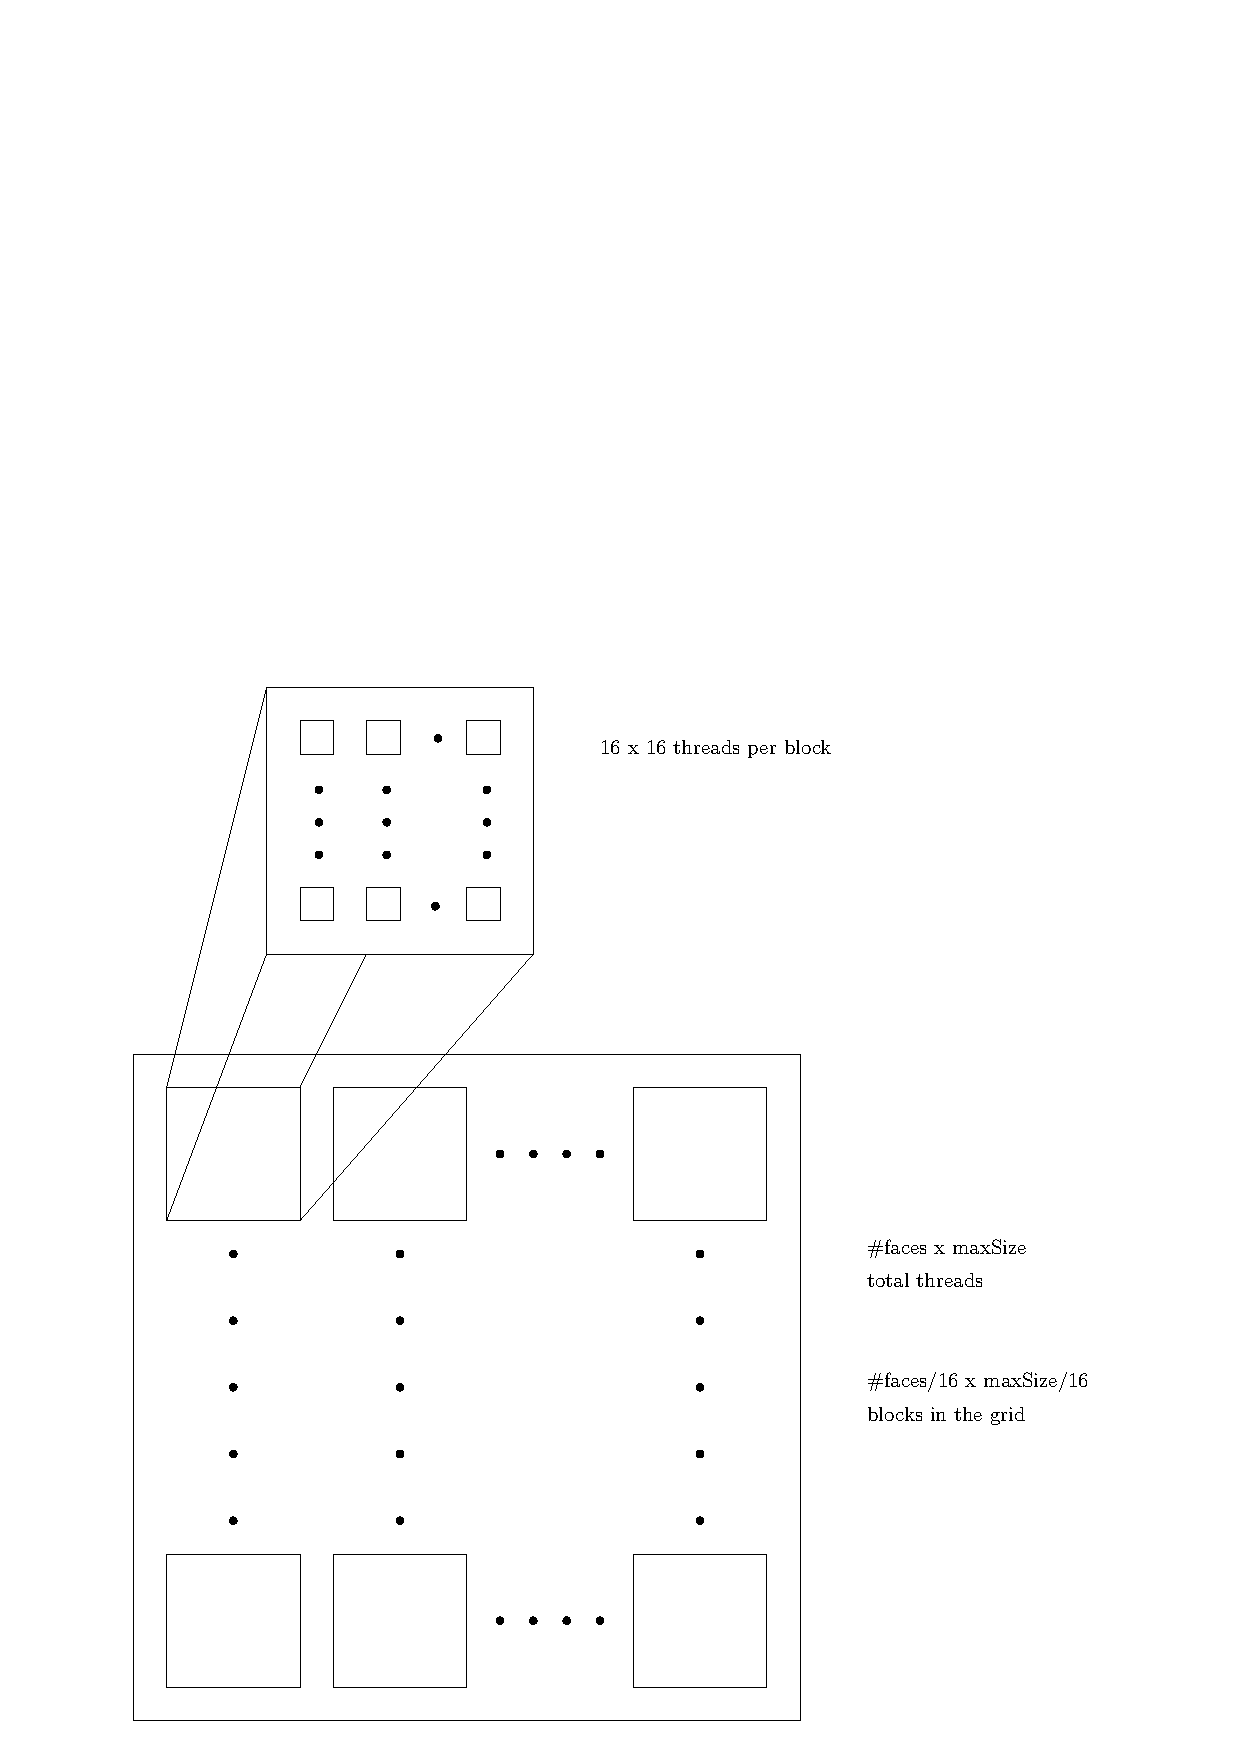
\includegraphics{Threads.pdf}
	\caption{Distribution of Threads in a block and total amount of threads in all blocks}
	\label{fig:threaddist}
\end{figure}

\subsection{Balancing of thread workload}
The edge-edge pairs are stored in an array of size \textit{nEdges * maxSize}, and for each edge all potential colliding edges are stored. This output array should also not contain any duplicate entries. The approach used in the CPU implementation solved this by checking the ids of the edges. Then, if the id of the first edge A is smaller than that of the second edge B, edge B is stored in the part of the array assigned to edge A. This results in a triangular adjacency matrix, as seen in table \ref{table:balance}. This is not a problem on a sequential CPU implementation, but in a parallel CUDA implementation this would lead to threads that have imbalanced workload distribution, resulting in overall performance degradation. Therefore we needed a method to balance this matrix. We did this using the following method.\\
\\
\indent \indent \textbf{if} $(A + B) \% 2 = 0$ \textbf{then} store at $min(A,B)$\\
\indent \indent \textbf{else} store at $max(A,B)$ \\
\\
This generally leads to a better distribution, as seen in table \ref{table:balance}.

\begin{table}[!htb]
    	\begin{subtable}{.5\linewidth}
		\centering
		\begin{tabular}{ c || c | c | c | c }
			1 & 2 & 3 & 4 & 5 \\
			2 & 3 & 4 & 5 \\
			3 & 4 & 5 & \\
			4 & 5 & & \\
			5 & & &\\
		\end{tabular}
		\caption{Old CPU balance}
	\end{subtable}%
    	\begin{subtable}{.5\linewidth}
		\centering        
		\begin{tabular}{ c || c | c | c | c }
			1 & 3 & 5 &  &  \\
			2 & 1 & 4 &  &\\
			3 & 2 & 5 &  &\\
			4 & 1 & 3 &  &\\
			5 & 2 & 4 &  &\\
		\end{tabular}
		\caption{New CUDA balance}
	\end{subtable} 
	\caption{Difference between balancing on a complete Edge-Edge adjacency matrix.}
	\label{table:balance}
\end{table}

\subsection{Parallel access to output arrays}
Since all the threads try to access the output arrays at the same time, we have to make sure that the state of the output arrays will stay consistent and make sure that calculations are done atomically. We came up with a smart trick to keep everything consistent: We need to use 2 arrays per output type, one to hold the output, and one to hold the number of collisions per vertex/edge, so that we can index the respective output array. CUDA has special atomic functions and the one we will use is called \texttt{atomicAdd()}. It will be used to increase the number of collisions in the count array. The function will return the result of the addition, thus the new index that can be used in the thread that called the atomic addition function. The trick is that the atomic add will be done atomically, so nothing can go wrong there, but the resulting index will be different for each of the parallel threads. They can now freely read/write in the output array at the given index, since no other thread will be given this index.

\subsection{Memory problems}
Unfortunately, after implementing everything, we could run the program for the \texttt{bunny.txt} data set, but all the other datasets required too much data in the memory of the GPU. First we will give an overview of the data we need, and then show how we have tried to address this problem. The data we need is listed below.

\begin{itemize}
	\item 2 arrays for the input: an array which contains sequentially for each face, at most \texttt{maxSize} faces for which a potential collision is detected, and another array which holds the actual amount of potential colliding faces, which is used to index the 1-dimensional input array.
	\item Mappings between faces/vertices/edges/3D-points: We have an array of \texttt{Face} objects, which contain the corresponding vertices and edges, an array of \texttt{Edge} objects, which contain the corresponding vertices, and an array of \texttt{Vertex} objects, which contain the actual coordinates of the points in the 3-dimentional space.
	\item Bounding boxes: for the vertex-face collisions, we use the already existing bounding boxes for the faces, since they are already calculated in the BVH. For the edge-edge pairs we can easily calculate the bounding boxes on the fly. We do need an extra array that contains for each face and integer that contains the index of that vertex' bounding box in the bounding boxes array.
	\item The output arrays: an array with for each vertex, at most \texttt{maxSize} faces for which a potential collision is detected, and an array which holds the actual amount of potential colliding vertices, used to index the former array. The other output array holds for each edge, at most \texttt{maxSize} edges for which a potential collision is deteced, and again a potential collision count array.
\end{itemize}

Now for the bigger data sets, this is too much data to hold in the GPU memory. The mappings and the bounding boxes are working data, so we need them in memory all the time to do the calculations. For the input arrays, we can split them and process them in batches, starting a new GPU kernel for each batch. We elaborate on this in the next section. Initially, we thought the same was possible for the output arrays, but since the input face-face pairs map to arbitrary vertices and edges, we need to have the full output arrays in memory all the time.\\

However, the sum of the size for the last 3 parts was already too big to fit in memory. Therefore we had to come up with extra solutions. The first one prunes the amount of bounding boxes we put in memory. We use the array that maps faces to box-indices, to create a new array that contains for each face the bounding box. This way, instead of having for each node in the BVH-tree a bounding box, we only use the leaves, which contain bounding boxes of the actual faces.\\

The second solution has to do with the variable \texttt{maxSize}, which was set to a way too high value. It's value was 5000, which means that for each face we have at most 5000 other faces with which in can potentially collide, and the same goes for the outputs (vertex-face and edge-edge). We tried decreasing the value to 500. While this saves a big amount of memory, since the space we reserved for face-face input, and vertex-face and edge-edge outputs, is now decreased by 90\%, we no longer get as precise results. Vertex-face pairs seem to be less effected by decreasing \texttt{maxSize}, than edge-edge pairs. Only in the \texttt{armadillo\_10000.txt} data set, we miss a minor 3 vertex-face pairs, but for nearly all models the edge-edge pairs are a lot less precise. For some data sets, like \texttt{lucy\_5000.txt} and \texttt{neptune\_10000.txt}, we started missing nearly half of the edge-edge pairs, when we prune the \texttt{maxSize}.

\subsection{Batches}
Even if the solutions for the memory problem in the previous section are not enough to get the program running, we can split the input array, so that we save some memory there. The downside is that we do a lot more smaller transfers from the host to the device, and we use less parallellism, since there is less data available for parallel execution in each batch. So there is a big tradeoff to be made here, but it might be neccessary to get the program running on the GPU, for certain data sets.\\

The idea of the batching is as follows: We keep on splitting the data in 2, so the first split gives us 2 half input arrays, the second split 4 kwarter input arrays and so on. As soon as we find that one part of the input array fits in memory with the rest of the data, we stop the splitting proces. We then transfer only reserve memory for and transfer the smaller part of the input onto the GPU. There are less threads processing at this point, but there is still parallellism. When all the threads have finished, we load the next part of the input in the GPU memory and make a new kernel call. This process is repeated until all the parts of the input have been processed, At the end of the input array we have to be careful, because the last remainder of the input does not necessarily have the same size as its predecessors. This means that we have to make sure that we only process the remaining part, and not the (no longer useful) data that is in the remaining space we reserved in GPU memory.

